\documentclass[FM,DP]{tulthesis}
\usepackage[czech]{babel}
\usepackage[utf8]{inputenc}

\usepackage{fontspec}
\usepackage{xunicode}
\usepackage{xltxtra}

\usepackage{listings}
\usepackage{color}

\usepackage[nottoc,notlot,notlof]{tocbibind}

\usepackage{amsmath}
\usepackage{graphicx}
\usepackage{float}

\usepackage{blindtext}

\newcommand{\verze}{0.9}
\newcommand{\argument}[1]{{\ttfamily\color{\tulcolor}#1}}
\newcommand{\prikaz}[1]{\argument{\textbackslash #1}}
\newenvironment{myquote}{\begin{list}{}{\setlength\leftmargin\parindent}\item[]}{\end{list}}
\newenvironment{listing}{\begin{myquote}\color{\tulcolor}}{\end{myquote}}
\sloppy

\TULtitle{TODO}{TODO}
\TULprogramme{N2612}{Elektrotechnika a informatika }{Electrical Engineering and Informatics }
\TULbranch{1802T007}{Informační technologie }{Information Technology}
\TULauthor{Ondřej Dlabola}
\TULsupervisor{}
\TULyear{2017}

\begin{document}

\ThesisStart{male}

\begin{abstractCZ}
TODO \Blindtext[2]

Klíčová slova: Reactive Streams, TODO

\end{abstractCZ}

\vspace{2cm}

\begin{abstractEN}
TODO \Blindtext[2]

Keywords: Reactive Streams, TODO

\end{abstractEN}

\tableofcontents

\clearpage

\chapter*{Úvod}
Který bude cca 1 strana spíše motivačně informačního charakteru, proč jsem tuto věc spáchal. \Blindtext[6]

\chapter{Reaktivní aplikace}

\section{Reactive manifesto}

\begin{figure}
\centering
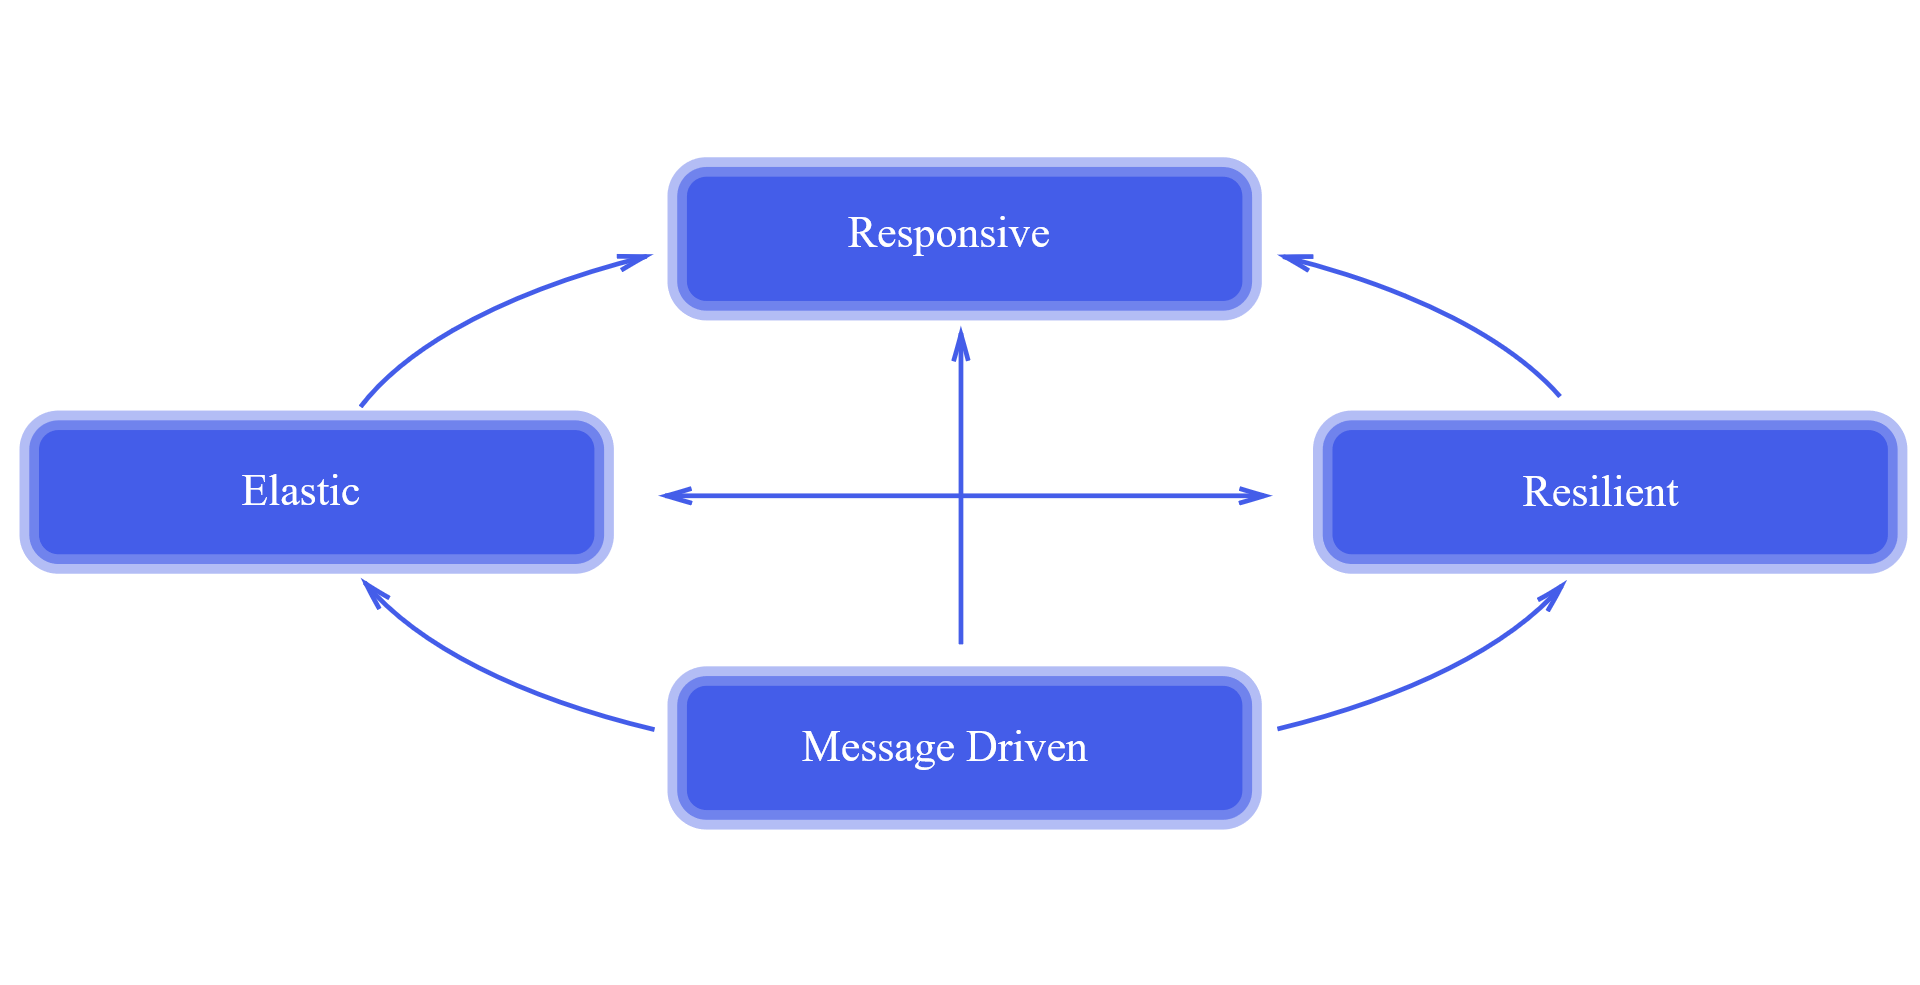
\includegraphics[scale=0.2]{img/reactive-traits}
\end{figure}

\subsection{Responsive}

\subsection{Resilient}

\subsection{Elastic}

\subsection{Message driven}

\section{Reaktivní proudy}

\chapter{Implementace a nástroje}

\section{Struktura}

\section{API}

\section{VertX}

\section{Cassandra}

\section{Docker}

\chapter{Testování a vylepšování}

\section{Gattling}

\section{Testování základního návrhu}

\section{Vylepšení pomocí feature A}

\section{Vylepšení pomocí feature B}

\chapter{Závěr}

\section{Zhodnocení}

\section{Možnosti k rozšíření}
	
\begin{thebibliography}{Per00}

\end{thebibliography}

\end{document}




